\chapter{Compressible Flow Solver}

\section{Synopsis}
The CompressibleFlowSolver allows us to solve
the unsteady compressible Euler and Navier-Stokes
equations for 1D/2D/3D problems using a discontinuous
representation of the variables. In the following we describe
both the compressible Euler and the Navier-Stokes equations.

\subsection{Euler equations}
The Euler equations can be expressed as a hyperbolic
conservation law in the form
\begin{equation}\label{eq:euler}
\frac{\partial \mathbf{q} }{\partial t} + \frac{\partial \mathbf{f}_i}{\partial x}
+ \frac{\partial \mathbf{g}_i}{\partial y} +
\frac{\partial \mathbf{h}_i}{\partial z} = 0,
\end{equation}
where $\mathbf{q} $ is the vector of the conserved variables,
$\mathbf{f}_i =  \mathbf{f}_i (\mathbf{q})$, $\mathbf{g}_i
= \mathbf{g}_i (\mathbf{q})$ and $\mathbf{h}_i =
\mathbf{h}_i (\mathbf{q})$ are  the vectors of the
inviscid fluxes
\begin{equation}
\mathbf{q} =\left\{
\begin{array}{c}
\rho \\
\rho u \\
\rho v \\
\rho w \\
E
\end{array} \right\}, \hspace{0.5 cm}
\mathbf{f}_i =\left\{
\begin{array}{c}
\rho u \\
p + \rho u^2 \\
\rho u v \\
\rho u w \\
u (E + p)
\end{array} \right\}, \hspace{0.5 cm}
\mathbf{g}_i =\left\{
\begin{array}{c}
\rho v \\
\rho u v \\
p + \rho v^2 \\
\rho v w \\
v (E + p)
\end{array} \right\}, \hspace{0.5 cm}
\mathbf{h}_i =\left\{
\begin{array}{c}
\rho w \\
\rho u w \\
\rho v w \\
p + \rho w^2 \\
w (E + p)
\end{array} \right\},
\label{Euler}
\end{equation}
where $\rho$ is the density, $u$, $v$ and $w$ are the velocity components in $x$, $y$ and
$z$ directions, $p$ is the pressure and $E$ is the total energy. In this work we considered
a perfect gas law for which the pressure is related to the total energy by the following expression
\begin{equation}
E = \frac{p}{\gamma - 1} + \frac{1}{2} \rho(u^2 + v^2 + w^2),
\label{energy}
\end{equation}
where $\gamma$ is the ratio of specific heats.
\subsection{Compressible Navier-Stokes equations}
The Navier-Stokes equations include the effects of fluid viscosity and heat
conduction and are consequently composed by an inviscid and a viscous
flux. They depend not only on the conserved variables but also, indirectly,
on their gradient. The second order partial differential equations for the
three-dimensional case can be written as:
\begin{equation}
\frac{\partial \mathbf{q} }{\partial t} +
\frac{\partial \mathbf{f}}{\partial x} +
\frac{\partial \mathbf{g}}{\partial y} +
\frac{\partial \mathbf{h}}{\partial z} = 0,
\end{equation}
where $\mathbf{q} $ is the vector of the conserved variables, $\mathbf{f} =
\mathbf{f} (\mathbf{q}, \nabla (\mathbf{q}))$,
$\mathbf{g}=  \mathbf{g} (\mathbf{q}, \nabla (\mathbf{q}))$ and $\mathbf{h} =
\mathbf{h} (\mathbf{q}, \nabla (\mathbf{q}))$
are the vectors of the  fluxes which can also be written as:
\begin{equation}
\begin{array}{l}
\mathbf{f} = \mathbf{f}_i - \mathbf{f}_v,
\mathbf{g} = \mathbf{g}_i - \mathbf{g}_v,
\mathbf{h} = \mathbf{h}_i - \mathbf{h}_v,
\end{array}
\end{equation}
where $\mathbf{f}_i$, $\mathbf{g}_i $ and $\mathbf{h}_i$ are the inviscid fluxes
of Eq. (\ref{Euler}) and $\mathbf{f}_v$, $\mathbf{g}_v $ and $\mathbf{h}_v$ are
the viscous fluxes which take the following form:
\begin{equation}
\begin{array}{c} \vspace{0.2 cm}
\mathbf{f}_v =\left\{
\begin{array}{c}
0 \\
\tau_{xx} \\
\tau_{yx} \\
\tau_{zx} \\
u \tau_{xx} + v \tau_{yx} + w \tau_{zx} + k T_x
\end{array} \right\},  \hspace{0.2 cm}
\mathbf{g}_v =\left\{
\begin{array}{c}
0 \\
\tau_{xy} \\
\tau_{yy} \\
\tau_{zy} \\
u \tau_{xy} + v \tau_{yy} + w \tau_{zy} + k T_y
\end{array} \right\}, \\ \vspace{0.2 cm}
\mathbf{h}_v =\left\{
\begin{array}{c}
0 \\
\tau_{xz} \\
\tau_{yz} \\
\tau_{zz} \\
u \tau_{xz} + v \tau_{yz} + w \tau_{zz} + k T_z
\end{array} \right\},
\end{array}
\label{viscous flux}
\end{equation}
where $\tau_{xx}$, $\tau_{xy}$, $\tau_{xz}$, $\tau_{yx}$, $\tau_{yx}$,
$\tau_{yy}$, $\tau_{yz}$, $\tau_{zx}$, $\tau_{zy}$ and $\tau_{zz}$ are
the components of the stress tensor\footnote{Note that we use Stokes
hypothesis $\lambda = -2/3$.}
\begin{equation}
\begin{array}{cc} \vspace{0.2 cm}
\tau_{xx} = 2 \mu \left( u_x - \frac{u_x + v_y + w_z}{3}  \right), &  \tau_{yy} =
2 \mu \left( v_y - \frac{u_x + v_y + w_z}{3}  \right), \\
\vspace{0.2 cm}\tau_{zz} = 2 \mu \left( w_z - \frac{u_x + v_y + w_z}{3}  \right),
& \tau_{xy} = \tau_{yx} = \mu(v_x + u_y), \\
\vspace{0.2 cm} \tau_{yz} = \tau_{zy} = \mu(w_y + v_z),  & \tau_{zx} = \tau_{xz} =
\mu(u_z + w_x). \\
\end{array}
\end{equation}
where $\mu$ is the dynamic viscosity calculated using
the Sutherland's law and $k$ is the thermal conductivity.

\subsection{Numerical discretisation}
In Nektar++ the spatial discretisation of the Euler and of the Navier-Stokes
equations is projected in the polynomial space via a discontinuous projection.
Specifically we make use either of the discontinuous Galerkin (DG) method
or the Flux Reconstruction (FR) approach.
In both the approaches the physical domain $\Omega$ is divided into a mesh
of $N$ non-overlapping elements $\Omega_{e}$ and the solution is allowed
to be discontinuous at the boundary between two adjacent elements.
Since the Euler as well as the Navier-Stokes equations are defined locally
(on each element of the computational domain), it is necessary to define
a term to couple the elements of the spatial discretisation in order to allow
information to propagate across the domain. This term, called numerical
interface flux, naturally arises from the discontinuous Galerkin formulation
as well as from the Flux Reconstruction approach.

For the advection term it is common to solve a Riemann problem at each
interface of the computational domain through exact or approximated Riemann
solvers. In Nektar++ there are different Riemann solvers, one exact and nine
approximated. The exact Riemann solver applies an iterative procedure to
satisfy conservation of mass, momentum and energy and the equation of
state. The left and right states are connected either with the unknown variables
through the Rankine-Hugoniot relations, in the case of shock, or the isentropic
characteristic equations, in the case of rarefaction waves. Across the contact
surface, conditions of continuity of pressure and velocity are employed.
Using these equations the system can be reduced to a non-linear algebraic
equation in one unknown (the velocity in the intermediate state) that is solved
iteratively using a Newton method. Since the exact Riemann solver gives
a solution with an order of accuracy that is related to the residual in the
Newton method, the accuracy of the method may come at high computational
cost. The approximated Riemann solvers are simplifications of the exact solver.

Concerning the diffusion term, the coupling between the elements is achieved
by using a local discontinuous Galerkin (LDG) approach as well as five different
FR diffusion terms.

The boundary conditions are also implemented by exploiting the numerical
interface fluxes just mentioned.
For a more detailed description of the above the interested reader can refer
to \cite{DeGMen14} and \cite{MenDeG14}.

\section{Usage}
\begin{lstlisting}[style=BashInputStyle]
CompressibleFlowSolver session.xml
\end{lstlisting}


\section{Session file configuration}
In the following we describe the session file configuration. Specifically we consider the
sections under the tag \inltt{<CONDITIONS>} in the session (.xml) file.
\subsection*{Parameters}
Under this section it is possible to set the parameters of the simulation.
\begin{lstlisting}[style=XmlStyle]
<PARAMETERS>
  <P> TimeStep            = 0.0000001                  </P>
  <P> FinTime             = 1.0                        </P>
  <P> NumSteps            = FinTime/TimeStep           </P>
  <P> IO_CheckSteps       = 5000                       </P>
  <P> IO_InfoSteps        = 1                          </P>
  <P> Gamma               = 1.4                        </P>
  <P> pInf                = 101325                     </P>
  <P> rhoInf              = 1.225                      </P>
  <P> TInf                = pInf/(287.058*rhoInf)      </P>
  <P> Twall               = pInf/(287.058*rhoInf)+15.0 </P>
  <P> uInf                = 147.4                      </P>
  <P> vInf                = 0.0                        </P>
  <P> wInf                = 0.0                        </P>
  <P> mu                  = 1e-5                       </P>
  <P> Pr                  = 0.72                       </P>
  <P> thermalConductivity = 0.02                       </P>
</PARAMETERS>
\end{lstlisting}
\begin{itemize}
\item \inltt{TimeStep} is the time-step we want to use;
\item \inltt{FinTime} is the final physical time at which we want our simulation to stop;
\item \inltt{NumSteps} is the equivalent of \inltt{FinTime} but instead of specifying the
physical final time we specify the number of time-steps;
\item \inltt{IO\_CheckSteps} sets the number of steps between successive checkpoint files;
\item \inltt{IO\_InfoSteps} sets the number of steps between successive info stats are printed
to screen;
\item \inltt{Gamma} ratio of the specific heats. Default value = 1.4;
\item \inltt{pInf} farfield pressure (i.e. $p_{\infty}$). Default value = 101325 $Pa$;
\item \inltt{rhoInf} farfield density (i.e. $\rho_{\infty}$). Default value = 1.225 $Kg/m^{3}$;
\item \inltt{TInf} farfield temperature (i.e. $T_{\infty}$). Default value = 288.15 $K$;
\item \inltt{Twall} temperature at the wall when isothermal boundary
conditions are employed (i.e. $T_{w}$). Default value = 300.15$K$;
\item \inltt{uint} farfield $X$-component of the velocity (i.e. $u_{\infty}$). Default value = 0.1 $m/s$;
\item \inltt{vInf} farfield $Y$-component of the velocity (i.e. $v_{\infty}$). Default value = 0.0 $m/s$;
\item \inltt{wInf} farfield $Z$-component of the velocity (i.e. $w_{\infty}$). Default value = 0.0 $m/s$;
\item \inltt{mu} dynamic viscosity (i.e. $\mu_{\infty}$). Default value = 1.78e-05 $Pa s$;
\item \inltt{Pr} Prandtl number. Default value = 0.72;
\item \inltt{thermalConductivity} thermal conductivity (i.e. $\kappa_{\infty}$). This can be set as an
 alternative to \inltt{Pr}, in which case the Prandtl number is calculated from $\kappa_{\infty}$
 (it is only possible to set one of them). By default, this is obtained from the Prandtl number;
\end{itemize}

\subsection*{Time Integration Scheme}
Under this section it is possible to set the time integration scheme
information.
\begin{lstlisting}[style=XmlStyle]
<TIMEINTEGRATIONSCHEME>
  <METHOD> RungeKutta </METHOD>
  <VARIANT> SSP </VARIANT>
  <ORDER> 3 </ORDER>
</TIMEINTEGRATIONSCHEME>
\end{lstlisting}
\begin{itemize}
\item \inltt{TimeIntegrationScheme} is the time-integration scheme we want to use.
Note that only an explicit discretisation is supported:
\begin{itemize}
\item \inltt{Method ForwardEuler, Order 1};
\item \inltt{Method RungeKutta, Variant SSP, Order 2};
\item \inltt{Method RungeKutta, Variant SSP, Order 3};
\item \inltt{Method RungeKutta, Order 4}.
\end{itemize}
\end{itemize}

\subsection*{Solver info}
Under this section it is possible to set the solver information.
\begin{lstlisting}[style=XmlStyle]
<SOLVERINFO>
  <I PROPERTY="EQType"                VALUE="NavierStokesCFE"      />
  <I PROPERTY="Projection"            VALUE="DisContinuous"        />
  <I PROPERTY="AdvectionType"         VALUE="WeakDG"               />
  <I PROPERTY="DiffusionType"         VALUE="LDGNS"                />
  <I PROPERTY="UpwindType"            VALUE="ExactToro"            />
  <I PROPERTY="ProblemType"           VALUE="General"              />
  <I PROPERTY="ViscosityType"         VALUE="Constant"             />
  <I PROPERTY="EquationOfState"       VALUE="IdealGas"             />
</SOLVERINFO>
\end{lstlisting}
\begin{itemize}
\item \inltt{EQType} is the tag which specify the equations we want solve:
\begin{itemize}
\item \inltt{NavierStokesCFE} (Compressible Navier-Stokes equations);
\item \inltt{EulerCFE} (Compressible Euler equations).
\item \inltt{IsentropicVortex} (Isentropic vortex test case).
\item \inltt{RinglebFlow} (Ringleb flow test case).
\end{itemize}
\item \inltt{Projection} is the type of projection we want to use:
\begin{itemize}
\item \inltt{DisContinuous}.\\
Note that the Continuous projection is not supported in the Compressible Flow Solver.
\end{itemize}
\item \inltt{AdvectionType} is the advection operator we want to use.
\begin{itemize}
\item \inltt{WeakDG} (classical DG in weak form);
\item \inltt{FRDG} (Flux-Reconstruction recovering nodal DG scheme);
\item \inltt{FRSD} (Flux-Reconstruction recovering a spectral difference (SD) scheme);
\item \inltt{FRHU} (Flux-Reconstruction recovering Huynh (G2) scheme);
\item \inltt{FRcmin} (Flux-Reconstruction with $c = c_{min}$);
\item \inltt{FRcinf} (Flux-Reconstruction with $c = \infty$).
\end{itemize}
Note that only \inltt{WeakDG} is fully supported, the other operators work only with quadrilateral elements ($2D$ or $2.5D$).
\item \inltt{DiffusionType} is the diffusion operator we want to use
for the Navier-Stokes equations:
\begin{itemize}
\item \inltt{LDGNS} (LDG with primitive variables. The penalty term is inversely proportional to the element size, proportional to the local viscosity for the momentum equations and to the thermal conductivity for the energy equation, and proportional to an optional parameter \inltt{LDGNSc11} which is by default set to one; proportionality to polynomial order can be manually imposed by setting the parameter \inltt{LDGNSc11} equal to $p^2$);
\item \inltt{LFRDGNS} (Flux-Reconstruction recovering nodal DG scheme);
\item \inltt{LFRSDNS} (Flux-Reconstruction recovering a spectral difference (SD) scheme);
\item \inltt{LFRHUNS} (Flux-Reconstruction recovering Huynh (G2) scheme);
\item \inltt{LFRcminNS} (Flux-Reconstruction with $c = c_{min}$);
\item \inltt{LFRcinfNS} (Flux-Reconstruction with $c = \infty$).
\end{itemize}
Note that only \inltt{LDGNS} is fully supported, the other operators work only with quadrilateral elements ($2D$ or $2.5D$).
\item \inltt{UpwindType} is the numerical interface flux (i.e. Riemann solver)
we want to use for the advection operator:
\begin{itemize}
\item \inltt{AUSM0};
\item \inltt{AUSM1};
\item \inltt{AUSM2};
\item \inltt{AUSM3};
\item \inltt{Average};
\item \inltt{ExactToro};
\item \inltt{HLL};
\item \inltt{HLLC};
\item \inltt{LaxFriedrichs};
\item \inltt{Roe}.
\end{itemize}
\item \inltt{ViscosityType} is the viscosity type we want to use:
\begin{itemize}
\item \inltt{Constant} (Constant viscosity);
\item \inltt{Variable} (Variable viscosity through the Sutherland's law.);
\end{itemize}
\item \inltt{EquationOfState} allows selecting an equation of state for
accounting for non-ideal gas behaviour:
\begin{itemize}
\item \inltt{IdealGas} (default option);
\item \inltt{VanDerWaals} (requires additional parameters \inltt{Tcrit} and \inltt{Pcrit});
\item \inltt{RedlichKwong} (requires additional parameters \inltt{Tcrit} and \inltt{Pcrit});
\item \inltt{PengRobinson} (requires additional parameters \inltt{Tcrit}, \inltt{Pcrit} and
\inltt{AcentricFactor});
\end{itemize}
\end{itemize}

\subsection*{Boundary conditions}
In this section we can specify the boundary conditions for our problem.
First we need to define the variables under the section \inltt{VARIABLES}.
For a 1D problem we have:
\begin{lstlisting}[style=XmlStyle]
<VARIABLES>
  <V ID="0"> rho  </V>
  <V ID="1"> rhou </V>
  <V ID="4"> E    </V>
</VARIABLES>
\end{lstlisting}

For a 2D problem we have
\begin{lstlisting}[style=XmlStyle]
<VARIABLES>
  <V ID="0"> rho  </V>
  <V ID="1"> rhou </V>
  <V ID="2"> rhov </V>
  <V ID="4"> E    </V>
</VARIABLES>
\end{lstlisting}

For a 3D problem we have:
\begin{lstlisting}[style=XmlStyle]
<VARIABLES>
  <V ID="0"> rho  </V>
  <V ID="1"> rhou </V>
  <V ID="2"> rhov </V>
  <V ID="3"> rhow </V>
  <V ID="4"> E    </V>
</VARIABLES>
\end{lstlisting}

After having defined the variables depending on the dimensions of the problem we want to solve
it is necessary to specify the boundary regions on which we want to define the boundary conditions:
\begin{lstlisting}[style=XmlStyle]
<BOUNDARYREGIONS>
  <B ID="0"> C[100] </B>
</BOUNDARYREGIONS>
\end{lstlisting}

Finally we can specify the boundary conditions on the regions specified under \inltt{BOUNDARYREGIONS}.
In the following some examples for a 2D problem:
\begin{itemize}
\item Slip wall boundary conditions:
\begin{lstlisting}[style=XmlStyle]
<BOUNDARYCONDITIONS>
  <REGION REF="0">
    <D VAR="rho"  USERDEFINEDTYPE="Wall" VALUE="0" />
    <D VAR="rhou" USERDEFINEDTYPE="Wall" VALUE="0" />
    <D VAR="rhov" USERDEFINEDTYPE="Wall" VALUE="0" />
    <D VAR="E"    USERDEFINEDTYPE="Wall" VALUE="0" />
  </REGION>
</BOUNDARYCONDITIONS>
\end{lstlisting}

\item No-slip wall boundary conditions:
\begin{lstlisting}[style=XmlStyle]
<BOUNDARYCONDITIONS>
  <REGION REF="0">
    <D VAR="rho"  USERDEFINEDTYPE="WallViscous" VALUE="0" />
    <D VAR="rhou" USERDEFINEDTYPE="WallViscous" VALUE="0" />
    <D VAR="rhov" USERDEFINEDTYPE="WallViscous" VALUE="0" />
    <D VAR="E"    USERDEFINEDTYPE="WallViscous" VALUE="0" />
  </REGION>
</BOUNDARYCONDITIONS>
\end{lstlisting}

\item Adiabatic wall boundary conditions:
\begin{lstlisting}[style=XmlStyle]
<BOUNDARYCONDITIONS>
  <REGION REF="0">
    <D VAR="rho"  USERDEFINEDTYPE="WallAdiabatic" VALUE="0" />
    <D VAR="rhou" USERDEFINEDTYPE="WallAdiabatic" VALUE="0" />
    <D VAR="rhov" USERDEFINEDTYPE="WallAdiabatic" VALUE="0" />
    <D VAR="E"    USERDEFINEDTYPE="WallAdiabatic" VALUE="0" />
  </REGION>
</BOUNDARYCONDITIONS>
\end{lstlisting}

In some cases we need to excite perturbations indide the boundary layer.
This can be achieved by setting part of the wall as a disturbance strip.
In the no-slip/adiabatic wall boundary conditions, if the \inltt{VALUE} is not
exact "0" but any expression, which can be time-dependent, the value of the
expression will be added to the ghost state of what it should be in the input
boundary conditions, and then generate a non-zero flus through the Riemann
solver. The following is an example to set a disturbance strip of amplitude
$A$, frequency $f$, and in the range of $[x_0, x_0+len]$ on a flat plate.
\begin{lstlisting}[style=XmlStyle]
  <BOUNDARYCONDITIONS>
    <REGION REF="0">
      <D VAR="rho"  USERDEFINEDTYPE="WallAdiabatic" VALUE="0" />
      <D VAR="rhou" USERDEFINEDTYPE="WallAdiabatic" VALUE="0" />
      <D VAR="rhov" USERDEFINEDTYPE="WallAdiabatic"
                    VALUE="A*sin(2*PI*f*t)*sin(2*PI*(x-x0)/len)
                            *(x>=x0)*(x<=(x0+len))"           />
      <D VAR="E"    USERDEFINEDTYPE="WallAdiabatic" VALUE="0" />
    </REGION>
  </BOUNDARYCONDITIONS>
\end{lstlisting}

\item Farfield boundary conditions (including inviscid characteristic boundary conditions):
\begin{lstlisting}[style=XmlStyle]
<BOUNDARYCONDITIONS>
  <REGION REF="0">
    <D VAR="rho"  VALUE="rhoInf" />
    <D VAR="rhou" VALUE="rhoInf*uInf" />
    <D VAR="rhov" VALUE="rhoInf*vInf" />
    <D VAR="E"
    VALUE="pInf/(Gamma-1)+0.5*rhoInf*(uInf*uInf+vInf*vInf+wInf*wInf)"/>
  </REGION>
</BOUNDARYCONDITIONS>
\end{lstlisting}

\item Pressure outflow boundary conditions:
\begin{lstlisting}[style=XmlStyle]
<BOUNDARYCONDITIONS>
  <REGION REF="0">
    <D VAR="rho"  USERDEFINEDTYPE="PressureOutflow" VALUE="0" />
    <D VAR="rhou" USERDEFINEDTYPE="PressureOutflow" VALUE="0" />
    <D VAR="rhov" USERDEFINEDTYPE="PressureOutflow" VALUE="0" />
    <D VAR="E"    USERDEFINEDTYPE="PressureOutflow" VALUE="pOut" />
  </REGION>
</BOUNDARYCONDITIONS>
\end{lstlisting}
where pOut is the target static pressure at the boundary.
\end{itemize}

\subsection*{Initial conditions and exact solution}
Under the two following sections it is possible to define the initial conditions and the exact solution (if existent).
\begin{lstlisting}[style=XmlStyle]
<FUNCTION NAME="InitialConditions">
  <E VAR="rho"    VALUE="rhoInf"/>
  <E VAR="rhou"   VALUE="rhoInf*uInf"   />
  <E VAR="rhov"   VALUE="rhoInf*vInf"   />
  <E VAR="E"
  VALUE="pInf/(Gamma-1)+0.5*rhoInf*(uInf*uInf+vInf*vInf+wInf*wInf)"/>
</FUNCTION>

<FUNCTION NAME="ExactSolution">
  <E VAR="rho"    VALUE="rhoInf"          />
  <E VAR="rhou"   VALUE="rhoInf*uInf"   />
  <E VAR="rhov"   VALUE="rhoInf*vInf"   />
  <E VAR="E"
  VALUE="pInf/(Gamma-1)+0.5*rhoInf*(uInf*uInf+vInf*vInf+wInf*wInf)"/>
</FUNCTION>
\end{lstlisting}

\section{Examples}
\subsection{Shock capturing}
Compressible flows can be characterised by abrupt changes in density within the flow domain often referred to as shocks. These discontinuities can lead to numerical instabilities (Gibbs phenomena). This problem is prevented by locally adding a diffusion term to the equations to damp the numerical oscillations.

\subsubsection{Non-smooth artificial viscosity model}
For the non-smooth artificial viscosity model the added artificial viscosity is constant in each element and discontinuous between the elements. The Euler system is augmented by an added Laplacian term on right hand side of equation \ref{eq:euler} \cite{persson2006sub}.
The diffusivity of the system is controlled by a variable viscosity coefficient $\varepsilon$.
For consistency $\varepsilon$ is proportional to the element size and inversely proportional to the polynomial order.
Finally, from physical considerations $\varepsilon$ needs to be proportional to the maximum characteristic speed of the problem.
The final form of the artificial viscosity is
\begin{equation}
  \varepsilon = \varepsilon_0 \frac{h}{p} \lambda_{max} S,
\end{equation}
where $S$ is a sensor.

As shock sensor, a modal resolution-based indicator is used
\begin{equation}\label{eq:sensor}
  s_e = log_{10}\left( \frac{\langle q - \tilde{q}, q - \tilde{q}  \rangle}{\langle q, q \rangle} \right) ,
\end{equation}
where $\langle \cdot, \cdot \rangle$ represents a $L^2$ inner product, $q$ and $\tilde{q}$ are the full and truncated expansions of a state variable (in our case density)
\begin{equation}
  q(x) = \sum_{i=1}^{N(P)} \hat{q}_i \phi_i , \quad \tilde{q}(x) = \sum_{i=1}^{N(P-1)} \hat{q}_i \phi_i ,
\end{equation}
then the constant element-wise sensor is computed as follows
\begin{equation}
   S_\varepsilon
=  \left \{ \begin{array}{lll}
    0 &	 \mbox{if} & s_e<s_0-\kappa \\
    \frac{1}{2}\left(1+\sin{\frac{\pi\left(s_e-s_0\right)}{2\kappa}}\right) &	\mbox{if} &	| s_e - s_0| \le \kappa\\
    1 &	 \mbox{if} & s_e > s_0+\kappa
      \end{array}
    \right.,
\end{equation}
where $s_0 = s_\kappa - 4.25\;log_{10}(p)$.

To enable the non-smooth viscosity model, the following line has to be added to the \inltt{SOLVERINFO} section:
\begin{lstlisting}[style=XmlStyle]
<SOLVERINFO>
  <I PROPERTY="ShockCaptureType"      VALUE="NonSmooth" />
<SOLVERINFO>
\end{lstlisting}
The diffusivity and the sensor can be controlled by the following parameters:
\begin{lstlisting}[style=XmlStyle]
<PARAMETERS>
<P> Skappa 	 	= -1.3                     </P>
<P> Kappa 	 	= 0.2                      </P>
<P> mu0 	  	= 1.0                      </P>
</PARAMETERS>
\end{lstlisting}

\begin{figure}[!htbp]
\begin{center}
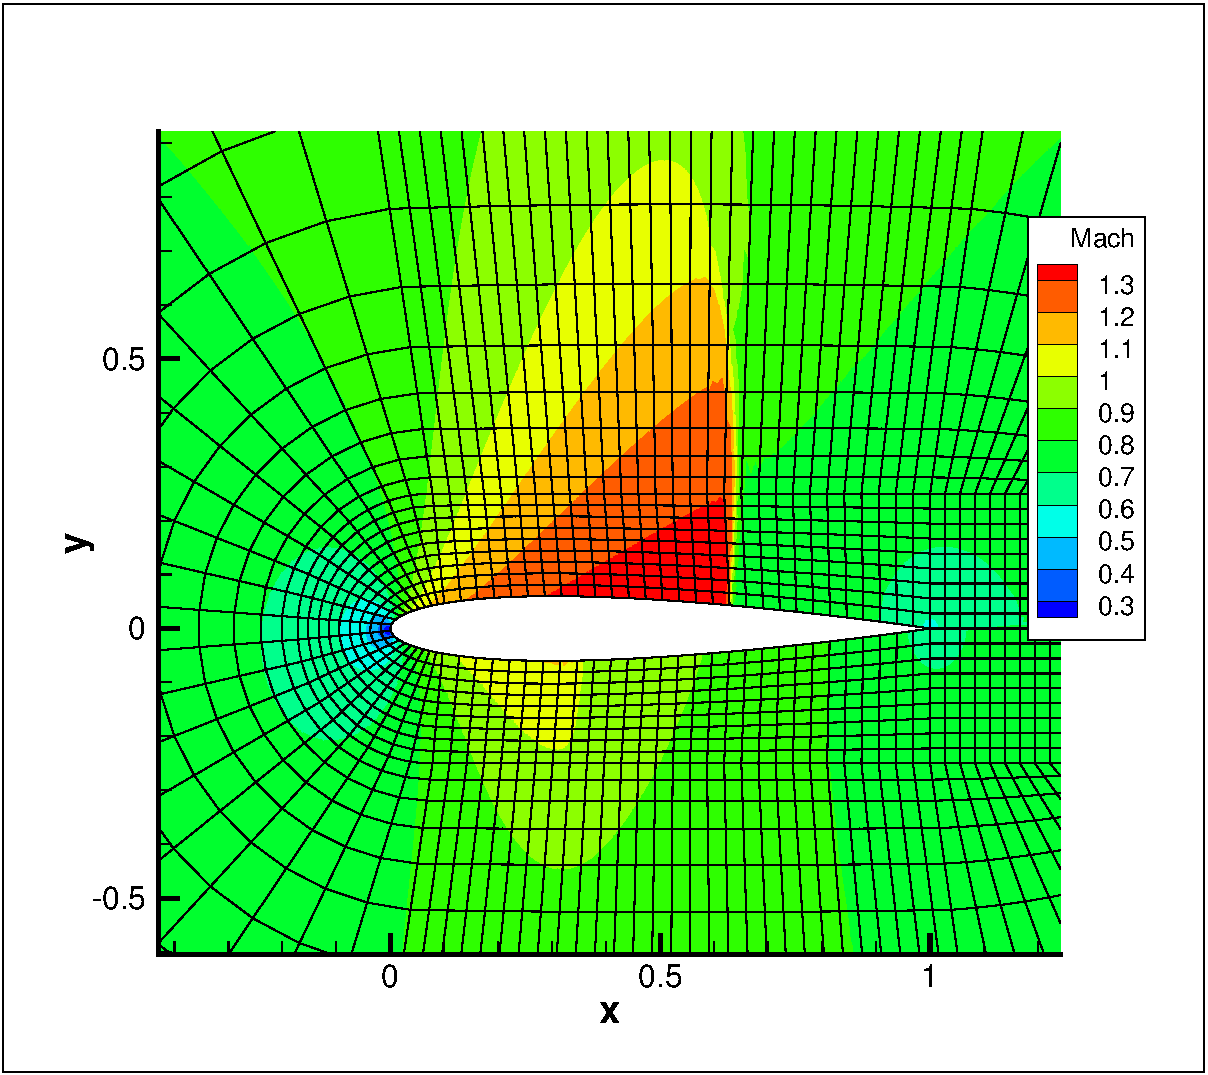
\includegraphics[width = 0.47 \textwidth]{img/Mach_P4.pdf}
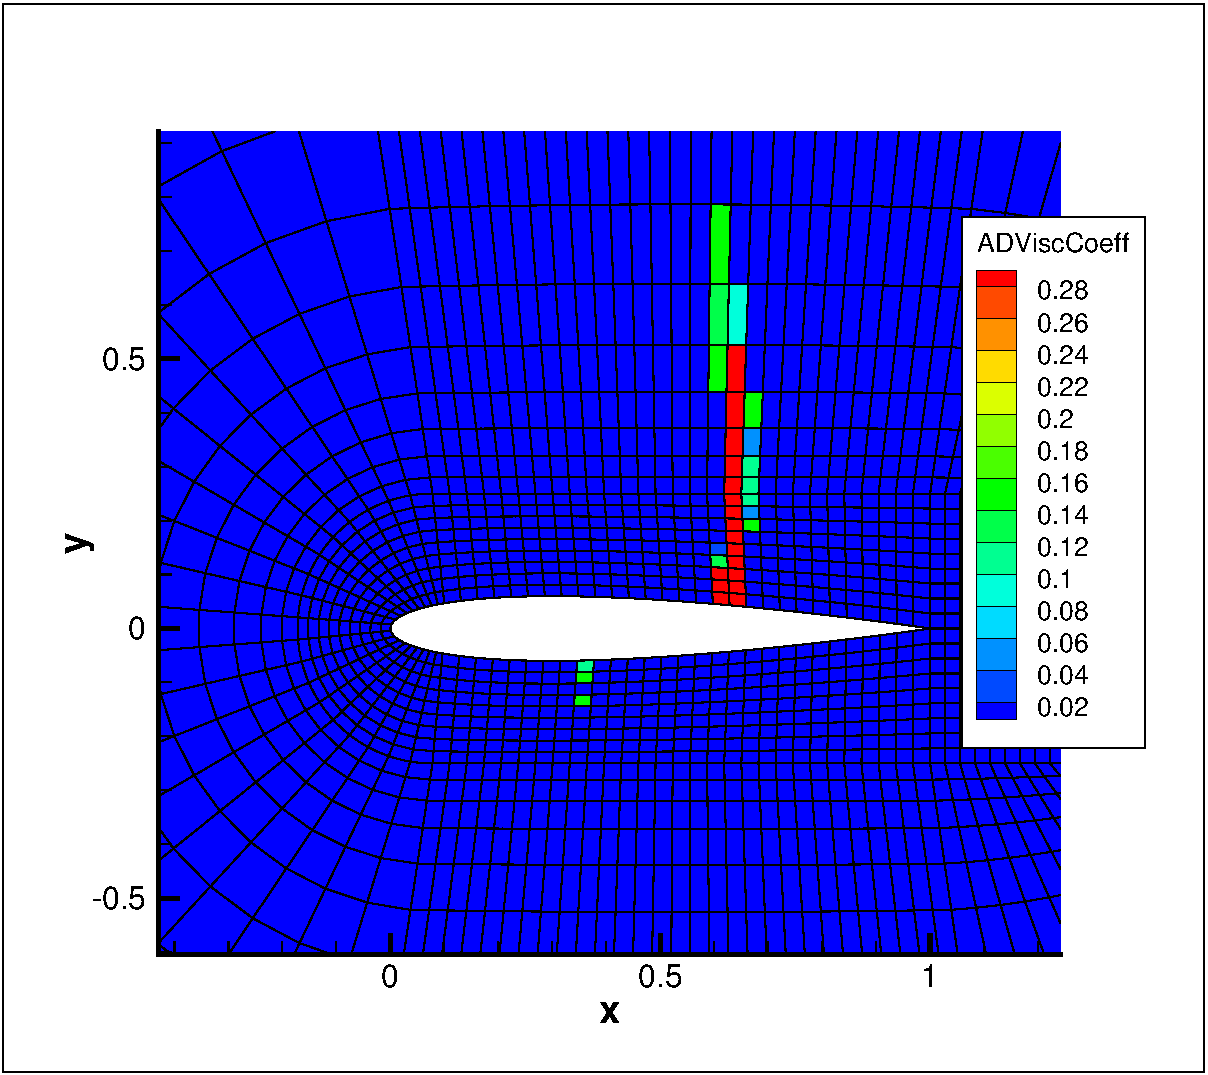
\includegraphics[width = 0.47 \textwidth]{img/ArtVisc_P4.pdf}
\caption{(a) Steady state solution for $M=0.8$ flow at $\alpha = 1.25^\circ$ past a NACA 0012 profile, (b) Artificial viscosity ($\varepsilon$) distribution}
\label{fig:}
\end{center}
\end{figure}

\subsection{Variable polynomial order}
A sensor based $p$-adaptive algorithm is implemented to optimise the computational cost and accuracy.
The DG scheme allows one to use different polynomial orders since the fluxes over the elements are determined using a Riemann solver and there is now further coupling between the elements. Furthermore, the initial $p$-adaptive algorithm uses the same sensor as the shock capturing algorithm to identify the smoothness of the local solution so it rather straightforward to implement both algorithms at the same time.\\
\\
The polynomial order in each element can be adjusted based on the sensor value that is obtained. Initially, a converged solution is obtained after which the sensor in each element is calculated. Based on the determined sensor value and the pre-defined sensor thresholds, it is decided to increase, decrease or maintain the degree of the polynomial approximation in each element and a new converged solution is obtained.\\
\begin{equation}\label{eq:pswitch}
  p_e =\left \{ \begin{array}{l}
    p_e-1\	\	\ \mbox{if}\		\	 s_e>s_{ds}\\
    p_e+1\	\	\ \mbox{if}\		\	 s_{sm }<s_e<s_{ds}\\
    p_e\	\	\	\	\	\	\	\	\	 \mbox{if}\		\ s_{fl}<s_e<s_{sm}\\
    p_e-1\	\	\ \mbox{if}\		\	 s_e<s_{fl}
    \end{array}
    \right.
\end{equation}
For now, the threshold values $s_e$, $s_{ds}$, $s_{sm}$ and $s_{fl}$ are determined empirically by looking at the sensor distribution in the domain. Once these values are set, two .txt files are outputted, one that has the composites called VariablePComposites.txt and one with the expansions called VariablePExpansions.txt. These values have to copied into a new .xml file to create the adapted mesh.
\subsection{De-Aliasing Techniques}
Aliasing effects, arising as a consequence of the nonlinearity of the
underlying problem, need to be address to stabilise the simulations. Aliasing
appears when nonlinear quantities are calculated at an insufficient number of
quadrature points. We can identify two types of nonlinearities:
\begin{itemize}
\item PDE nonlinearities, related to the nonlinear and quasi-linear fluxes.
\item Geometrical nonlinearities, related to the deformed/curves meshes.
\end{itemize}
We consider two de-aliasing strategies based on the concept of consistent integration:

\begin{itemize}
\item Local dealiasing: It only targets the PDE-aliasing sources, applying a consistent integration of them locally.
\item Global dealiasing: It targets both the PDE and the geometrical-aliasing sources. It requires a richer quadrature order to consistently integrate the nonlinear fluxes, the geometric factors, the mass matrix and the boundary term.
\end{itemize}

Since Nektar++ tackles separately the PDE and geometric aliasing during the
projection and solution of the equations, to consistently
integrate all the nonlinearities in the compressible
NavierStokes equations, the quadrature points should
be selected based on the maximum order of the nonlinearities:
\begin{equation}
Q_{min}= P_{exp}+\frac{max(2P_{exp},P_{geom})}{2} + \frac{3}{2}
\end{equation}

where $Q_{min}$ is the minimum required number of quadrature
points to exactly integrate the highest-degree of nonlinearity,
$P_{exp}$ being the order of the polynomial expansion and $P_{geom}$
being the geometric order of the mesh. Bear in mind that we are
using a discontinuous discretisation, meaning that aliasing
effect are not fully controlled, since the boundary terms
introduce non-polynomial functions into the problem.

To enable the global de-aliasing technique, modify the number of quadrature
points by:

\begin{lstlisting}[style=XmlStyle]
<E COMPOSITE="[101]"
   BASISTYPE="Modified_A,Modified_A"
   NUMMODES="7,7"
   POINTSTYPE="GaussLobattoLegendre,GaussLobattoLegendre"
   NUMPOINTS="14,14"
   FIELDS="rho,rhou,rhov,E"
/>
\end{lstlisting}

where \inltt{NUMMODES} corresponds to $P$+1, where $P$ is the order of the polynomial
used to approximate the solution. \inltt{NUMPOINTS} specifies the number of quadrature
points.
